
%(BEGIN_QUESTION)
% Copyright 2010, Tony R. Kuphaldt, released under the Creative Commons Attribution License (v 1.0)
% This means you may do almost anything with this work of mine, so long as you give me proper credit

An Allen-Bradley SLC 500 PLC is used to control an air compressor, using an across-the-line motor starter.  All 480 volt power wiring has been omitted for simplicity:

$$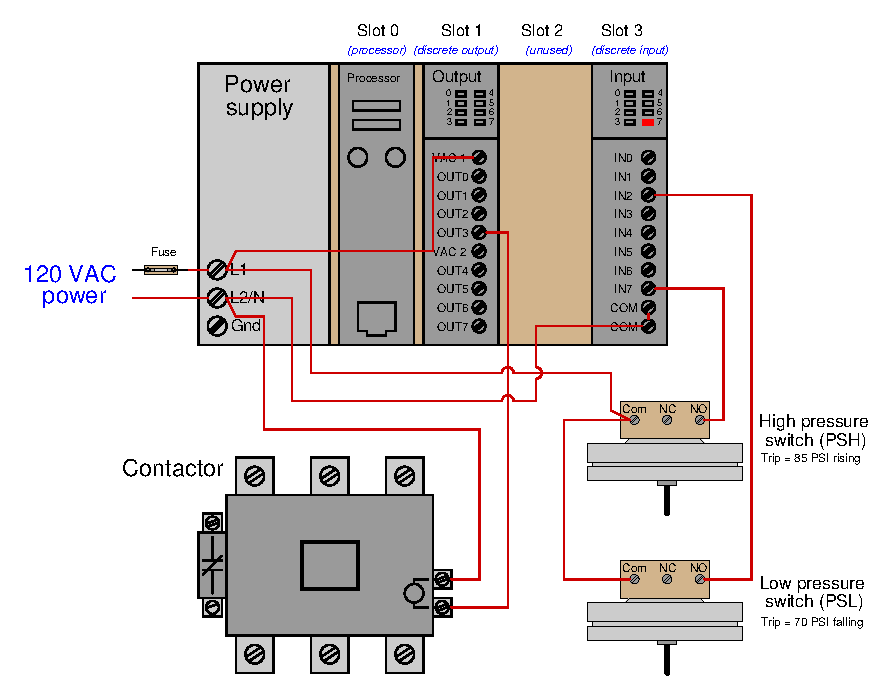
\includegraphics[width=15.5cm]{i02254x01.eps}$$

The system is broken, though: the compressor refuses to start even though the air tank is empty (no air pressure).  You have no test equipment with you -- all you have is what you see in the above illustration.

\vskip 10pt

Identify the likelihood of each specified fault in this system.  Consider each fault one at a time (i.e. no coincidental faults), determining whether or not each fault could independently account for {\it all} observations and symptoms in this circuit.

% No blank lines allowed between lines of an \halign structure!
% I use comments (%) instead, so that TeX doesn't choke.

$$\vbox{\offinterlineskip
\halign{\strut
\vrule \quad\hfil # \ \hfil & 
\vrule \quad\hfil # \ \hfil & 
\vrule \quad\hfil # \ \hfil \vrule \cr
\noalign{\hrule}
%
% First row
{\bf Fault} & {\bf Possible} & {\bf Impossible} \cr
%
\noalign{\hrule}
%
% Another row
Open wire between PSL and IN2 terminal &  &  \cr
%
\noalign{\hrule}
%
% Another row
Open wire between PSH and IN7 terminal &  &  \cr
%
\noalign{\hrule}
%
% Another row
Open contactor coil &  &  \cr
%
\noalign{\hrule}
%
% Another row
Shorted contactor coil &  &  \cr
%
\noalign{\hrule}
%
% Another row
PSL stuck (as though $P >$ 70 PSI) &  &  \cr
%
\noalign{\hrule}
%
% Another row
PSH stuck (as though $P >$ 85 PSI) &  &  \cr
%
\noalign{\hrule}
%
% Another row
Failed input card &  &  \cr
%
\noalign{\hrule}
%
% Another row
Failed output card &  &  \cr
%
\noalign{\hrule}
%
% Another row
PLC program halted &  &  \cr
%
\noalign{\hrule}
%
% Another row
Blown fuse &  &  \cr
%
\noalign{\hrule}
} % End of \halign 
}$$ % End of \vbox

\vfil 

\underbar{file i02254}
\eject
%(END_QUESTION)





%(BEGIN_ANSWER)

This is a graded question -- no answers or hints given!

%(END_ANSWER)





%(BEGIN_NOTES)

Looking at the LED indicators on the input cards of this PLC, we see that channel 7 on the discrete input card is lit.  This channel is connected to the high-pressure switch (PSH), which is itself a normally-open (NO) switch.  Being normally-open, the PSH should be open when at rest (low pressure) and closed when the pressure exceeds its trip setting (85 PSI).  Thus, the PLC ``thinks'' the pressure is greater than the high trip point of 85 PSI.  This may be due to a failure inside the high-pressure switch (PSH), or perhaps a failure inside the PLC's input card on that channel (i.e. reporting an energized condition when there really is no power present at the IN7 terminal).

\vskip 10pt

With the PLC being told that the pressure exceeds the high trip point, it will not try to run the compressor motor, which is why the output channel 3's LED is unlit.  Therefore, there is no problem with any component in the output circuitry -- the motor isn't turning on for the simple reason that the PLC is not even trying to turn it on.  Neither should we expect to find any problem with the PLC program itself.

\vskip 10pt

The other pressure switch (PSL) is also a normally-open device, and we see that its LED indicator is off, showing us that this switch ``thinks'' the pressure is below the PSL trip point of 70 PSI.  We have been told that the air tank is indeed empty, and so it would seem the PSL pressure switch is telling us the truth.  Therefore, we may conclude there is no problem to be found in any portion of the PSL circuitry.

% No blank lines allowed between lines of an \halign structure!
% I use comments (%) instead, so that TeX doesn't choke.

$$\vbox{\offinterlineskip
\halign{\strut
\vrule \quad\hfil # \ \hfil & 
\vrule \quad\hfil # \ \hfil & 
\vrule \quad\hfil # \ \hfil \vrule \cr
\noalign{\hrule}
%
% First row
{\bf Fault} & {\bf Possible} & {\bf Impossible} \cr
%
\noalign{\hrule}
%
% Another row
Open wire between PSL and IN2 terminal &  & $\surd$ \cr
%
\noalign{\hrule}
%
% Another row
Open wire between PSH and IN7 terminal &  & $\surd$ \cr
%
\noalign{\hrule}
%
% Another row
Open contactor coil &  & $\surd$ \cr
%
\noalign{\hrule}
%
% Another row
Shorted contactor coil &  & $\surd$ \cr
%
\noalign{\hrule}
%
% Another row
PSL stuck (as though $P >$ 70 PSI) &  & $\surd$ \cr
%
\noalign{\hrule}
%
% Another row
PSH stuck (as though $P >$ 85 PSI) & $\surd$ &  \cr
%
\noalign{\hrule}
%
% Another row
Failed input card & ? &  \cr
%
\noalign{\hrule}
%
% Another row
Failed output card &  & $\surd$ \cr
%
\noalign{\hrule}
%
% Another row
PLC program halted &  & $\surd$ \cr
%
\noalign{\hrule}
%
% Another row
Blown fuse &  & $\surd$ \cr
%
\noalign{\hrule}
} % End of \halign 
}$$ % End of \vbox

A more advanced analysis of the possible faults may shed doubt on an input card failure.  Many PLCs' input card LED indicator lights are wired in such a way that the LED only illuminates when the respective terminal on the card receives real power from a field sensor.  If the card in question is designed this way, then the illuminated IN7 LED represents the presence of real power at that input channel, which would mean the only possible fault could be a stuck PSH switch.  

On the other hand, some other PLC input card designs are such that the LED indicator lights are powered by the PLC microprocessor in response to sensing power at the respective channel terminal.  If this is the case, then it is possible that a component within the card has failed in such a way to fool the PLC's microprocessor into ``thinking'' that there is power at terminal IN7 when in fact there is not, causing the LED for IN7 to light up even with no real power at terminal IN7.

Since we were not given any detailed information about the design of the input card on this PLC, we cannot tell which case applies to this scenario.  Therefore, the input card being failed is ``possible'' only in the sense that that input card might be the type where its LEDs are powered by the microprocessor and not by real power at the input terminal, and this would fit the symptoms seen in this scenario.

%INDEX% PLC, troubleshooting: motor start/stop control circuit

%(END_NOTES)

